\chapter{Modeling}

\begin{figure}[hbtp]
	\centering
	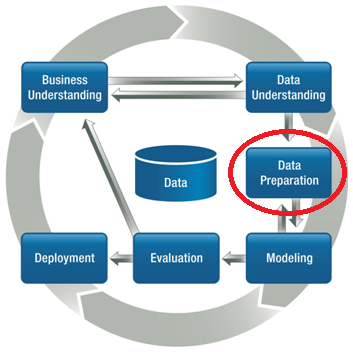
\includegraphics[width=0.5\textwidth]{./images/CRISPDM_3.png}
	\caption{CRISP-DM - Modeling}
	\label{CRISPDM_4}
\end{figure}

\section{Tecnica di Modeling}
Ai fini della classificazione, si è deciso di modellare il dataset realizzando un albero di decisione funzionale. In particolare si è utilizzato l'algoritmo \textbf{FT} (\textit{\textbf{F}unctional \textbf{T}ree}).

\section{Rappresentazione del Modello}
L'algoritmo Functional Tree è un algoritmo di classificazione basato sulla costruzione di alberi 'funzionali', i quali potrebbero avere funzioni di regressione logistica ai nodi e/o alle foglie interne. L'algoritmo, cosi come descritto in \cite{Gama2004}, è in grado di gestire:
\begin{itemize}
	\item variabili target (binarie o multi-classe);
	\item attributi numerici;
	\item attributi nominali;
	\item missing values.
\end{itemize}
%Classifier for building 'Functional trees', which are classification trees  that could have logistic regression functions at the inner nodes and/or leaves. The algorithm can deal with binary and multi-class target variables, numeric and nominal attributes and missing values.\cite{Gama2004}

\paragraph{Alberi Funzionali}
Dato un set di esempi e un costruttore di attributi, l'algoritmo generale usato per la costruzione dell'albero funzionale è mostrato di seguito. Questo algoritmo è molto simile a molti altri, fatta eccezione nella fase di costruzione (Fasi 3 e 4). Qui viene creata una nuova funzione e mappata ai nuovi attributi creati. Ci sono alcuni aspetti di questo algoritmo che devono essere esplicitati. Nella fase 3, il modello viene costruito usando la funzione costruttore. Questo viene fatto usando solo gli esempi che ricadono in questo nodo. Successivamente, nella fase 4, il modello viene mappato ai nuovi attributi. La funzione costruttore deve essere o un classificatore o un regressore in base alla tipologia di problema. Il numero dei nuovi attributi da creare, sarà uguale al numero delle classi che si hanno a disposizione; Infine, la funzione costruttore è mappata ad un nuovo attributo. Nella fase 3, ogni nuovo attributo è computato come valore predetto dalla funzione costruita per ogni esempio. In caso di classificazione, ogni nuovo attributo-valore sarà la probabilità che quell'esempio appartenga ad una delle classi date dal modello costruito.
Il valore di ogni nuovo attributo viene valutato usando la funzione di merito di un albero univariato tenendo conto sempre dei valori originali degli attributi (Fase 7). Il modello costruito dall'algoritmo ha due tipi di nodi decisionali: Quelli basati sul test di uno degli attributi originali, e quelli basati sul valore della funzione costruttore. Quando si usa un modello lineare generalizzato (GLM) come costruttore di attributi, ogni nuovo attributo è una combinazione lineare degli attributi originali. I nodi decisionali basati sugli attributi costruiti, definiscono un piano di decisione multivariato.

%\begin{figure}[hbtp]
%	\centering
%	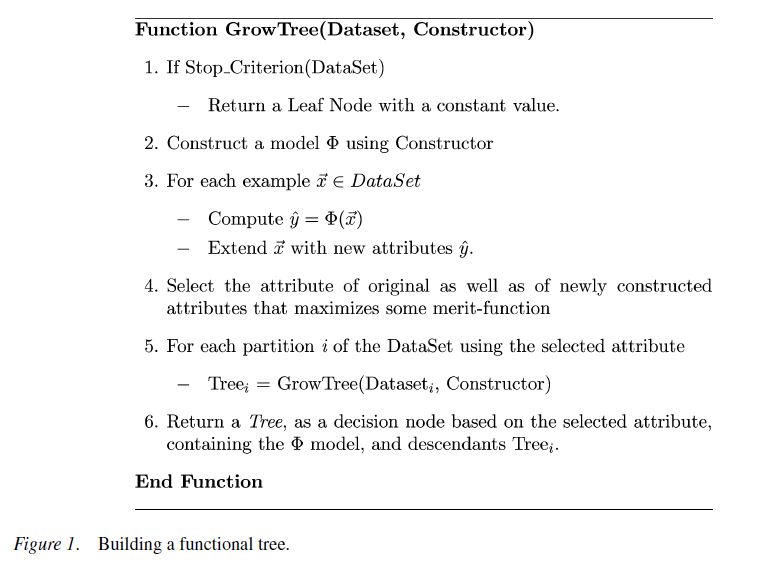
\includegraphics[width=0.9\textwidth]{./images/FunctionGrowTree.JPG}
%	\caption{Function GrowTree}
%\end{figure}

\lstset{style=customAlg}
\begin{algorithm}
	\caption{Function GrowTree(Dataset, Constructor)}
	\begin{lstlisting}
		If $Stop\_Criterion(DataSet)$
			Return a Leaf Node with a constant value.
		Construct a model $\Phi$ using Constructor
		For each example $\vec{x} \in DataSet$
			Compute $\hat y = \Phi(\vec{x})$
			Extend $\vec{x}$ with new attributes $\hat y$.
		Select the attribute of original as well as of newly constructed attributes that maximizes some merit-function
		For each partition $i$ of the DataSet using the selected attribute
			$Tree_{i} = GrowTree (Dataset_{i},Constructor)$
		Return a $Tree$, as a decision node based on the selected attribute, contaning the $\Phi$ model, and descendants $Tree_{i}$.
	\end{lstlisting}
\end{algorithm}

%\textbf{Function GrowTree(Dataset, Constructor)}
%\begin{enumerate}
%	\item If $Stop\_Criterion(DataSet)$
%	\begin{itemize}
%		\item Return a Leaf Node with a constant value.
%	\end{itemize}
%	\item Construct a model $\Phi$ using Constructor
%	\item For each example $\vec{x} \in DataSet$
%	\begin{itemize}
%		\item Compute $\hat y = \Phi(\vec{x})$
%		\item Extend $\vec{x}$ with new attributes $\hat y$.
%	\end{itemize}
%	\item Select the attribute of original as well as of newly constructed attributes that maximizes some merit-function \label{selection}
%	\item For each partition $i$ of the DataSet using the selected attribute
%	\begin{itemize}
%		\item $Tree_{i} = GrowTree (Dataset_{i},Constructor)$
%	\end{itemize}
%	\item Return a $Tree$, as a decision node based on the selected attribute, contaning the $\Phi$ model, and descendants $Tree_{i}$.
%\end{enumerate}
%\textbf{End Function}

Una volta creato l'albero, si passa alla fase di potatura. L'algoritmo generale di potatura verrà mostrato in seguito. L'albero viene visitato usando un approccio bottom-up (Post-visita). Per ogni nodo non foglia vengono stimati due valori quantitativi: 
\begin{itemize}
	\item Errore statico;
	\item Errore di Backed-up.
\end{itemize}
L'\textbf{errore statico} è la stima dell'errore se il nodo fosse foglia.
L'\textbf{errore di backed-up} è la somma pesata della stima degli errori di tutti i sotto alberi del nodo corrente. La stima dell'errore di ogni ramo è pesato usando la probabilità che un esempio appartenga al ramo. Se l'errore di backed-up è più grande o uguale all'errore statico, il nodo verrà sostituito da una foglia avente come valore, il valore dato dalla classe di maggioranza del nodo. L'aspetto fondamentale dell'algoritmo di potatura è l'errore stimato nella fase 1. Ad ogni nodo, sarà necessario stimare la probabilità dell'errore dato l'errore nel campione degli esempi che ricadono in questo nodo. La probabilità dell'errore non può essere determinato esattamente. Per un dato livello di confidenza, otteniamo un intervallo di confidenza [$L_{cf}$; $U_{cf}$] con una probabilità di 1-$cf$ che contenga l'errore reale. Cosi come in \cite{Quinlan:1993a}, il limite superiore dell'intervallo di confidenza ($U_{cf}$) sta ad indicare la \emph{stima pessimistica} dell'errore reale. L'intervallo di confidenza per l'errore dipende dalla funzione di perdita usato. In caso di classificazione, con perdita 0-1, l'errore segue una distribuzione Binomiale (\cite{mitchellbook}). Per ogni nodo, il limite superiore dell'intervallo di confidenza si ottiene dall'errore di campionamento della distribuzione.
Una procedura simile viene usata per stimare l'errore di costruzione. (Fase 4)

% \begin{figure}[hbtp]
% 	\centering
% 	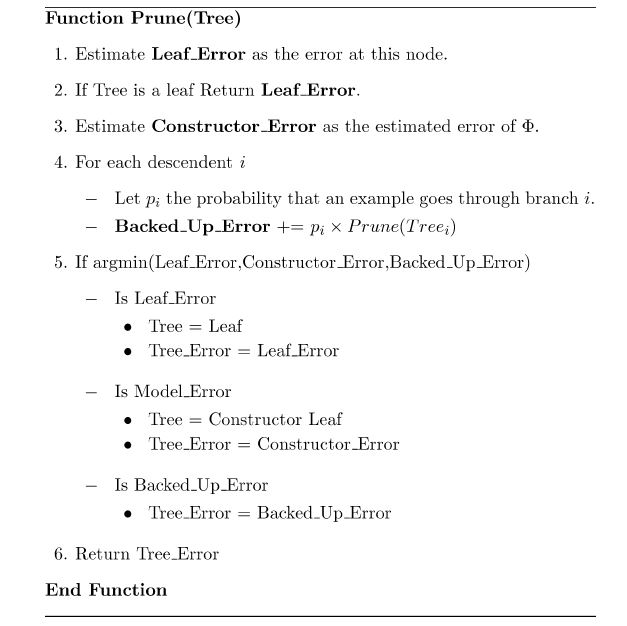
\includegraphics[width=0.5\textwidth]{./images/FunctionGrowTreePrune.JPG}
% 	\caption{Function GrowTree Prune}
% \end{figure}

\begin{algorithm}
	\caption{Function Prune (Tree)}
	\begin{lstlisting}
		Estimate Leaf_Error as the error at this node
		If Tree is leaf 
			Return Leaf_Error
		Estimate Constructor_Error as the estimated error of $\Phi$
		For each descendent $i$
			Let $p_i$ the probability that an example goes through branch $i$
			Backed_Up_Error $+= p_i \times Prune \left(Tree_i\right)$
		If argmin (Leaf_Error, Constructor_Error, Backed_up_error)
			Is Leaf_Error
				Tree = Leaf
				Tree_Error = Leaf_Error
			Is Model Error
				Tree = Constructor Leaf
				Tree_Error = Constructor_Error
			Is Backed_Up_Error
				Tree_Error = Backed_Up_Error
	\end{lstlisting}
\end{algorithm}

L'algoritmo di potatura produce due diversi tipi di foglie: foglie ordinarie che predicono una costante, e foglie costruttrici in grado di predire il valore della funzione costruttrice appresa (in fase di crescita) a quel nodo.
Si ottengono cosi due modelli concettualmente differenti in base a questa differenziazione descritti in seguito.

%Given a set of examples and an attribute constructor, the general algorithm used to build a
%functional tree is presented in figure 1. This algorithm is similar to many others, except in the constructive phase (steps 2 and 3). Here a function is built and mapped to new attributes.
%There are some aspects of this algorithm that should be made explicit. In step 2, a model
%is built using the constructor function. This is done using only the examples that fall at
%this node. Later, in step 3, the model is mapped to new attributes. The constructor function
%should be a classifier or a regressor depending on the type of the problem. In the former
%the number of new attributes is equal to the number of classes(At different nodes the system considers different number of classes depending on the class distribution of the
%examples that fall at this node.), in the latter the constructor
%function is mapped to one new attribute. In step 3, each new attribute is computed as the
%value predicted by the constructed function for each example. In the classification setting,each new attribute-value is the probability that the example belongs to one class given by the constructed model.
%The merit of each new attribute is evaluated using the merit-function of the univariate tree, and in competition with the original attributes (step 4). The model built by our algorithm has two types of decision nodes: those based on a test of one of the original attributes,and those based on the values of the constructor function. When using generalized linear models (GLM) as the attribute constructor, each new attribute is a linear combination of the original attributes. Decision nodes based on constructed attributes define a multivariate decision surface. 
%Once a tree has been built, it is pruned back. The general algorithm to prune the tree is presented in figure 2. The tree is traversed using a bottom-up, post-order strategy. For each non-leaf node two quantities are estimated: the static error and the backed-up error. Static error is an estimation of the error as if the node were a leaf. Backed-up error is the weighted sum of the estimation of the errors of all subtrees of the current node. The estimation of the error of each branch is weighted by the probability that an example follows the branch. If backed-up error is greater or equal than static error, then the node is replaced by a leaf with the majority class of the node.
%The fundamental aspect of the pruning algorithm is the error estimation in step 1. At each node, we need to estimate the probability of error given the error in the sample of examples that fall at this node. The probability of error cannot be determined exactly. For a given confidence level we can obtain a confidence interval [Lcf ;Ucf ] that with probability 1−cf contains the true error. 
%As in Quinlan (1993a), we use the upper limit of the confidence
%interval Ucf as a pessimistic estimation for the true error.
%The confidence interval for the error depends on the loss-function used. In classification problems, and under the 0-1 loss, the error is governed by a Binomial distribution (Mitchell,1997). In regression problems, and for the squared error loss the variance of the error for a given example follows a χ2 distribution. For a set of examples the sum of χ2 can be approximated using a Normal distribution (Bhattacharyya \& Johnson, 1977). For each node, the upper limit of the confidence interval is obtained from the sample error using
%the appropriate distribution. A similar procedure is used to estimate the constructor error(step 3).
%The pruning algorithm produces two different type of leaves: ordinary leaves that predict a constant, and constructor leaves that predict the value of the constructor function learned (in the growing phase) at this node.
%We obtain different conceptual models by simplifying our algorithm. Two interesting simplifications are described in the following sub-sections.

\paragraph{Alberi funzionali ai soli nodi foglia}
\label{Alberi funzionali ai soli nodi foglia}
Utilizzando l'approccio FT-Leaves, il modello funzionale non viene utilizzato nei test per effettuare lo splitting, ma solo ed esclusivamente nelle foglie. In questo approccio, si restringe la selezione degli attributi di test, ai soli attributi originali.
Questo è l'approccio utilizzato ad esempio nell'M5 di Quinlan \cite{Quinlan93combininginstance-based}, e nel sistema NBtree \cite{Kohavi1996}. 
Tuttavia, ad ogni nodo viene costruita la funzione costruttore che verrà poi utilizzata nella fase di pruning dell'albero. In questo modo, tutti i nodi decisionali sono basati sugli attributi di partenza. I nodi foglia potrebbero contenere il modello costruttore. Un nodo foglia conterrà il modello costruttore se e solo se nell'algoritmo di pruning l'errore stimato del modello costruttore è inferiore sia all'errore di backed-up che all'errore statico. Un albero funzionale FT-Leaves divide lo spazio di input in iper-rettagoli. I dati in ogni regione vengono adattati usando la funzione costruttore.
%Nevertheless we still build, at each node, the constructor function. The model built by the constructor function is used later in the pruning phase. In this way, all decision nodes are based on the original attributes. Leaf nodes could contain a constructor model. A leaf node contains a constructor model if and only if in the pruning algorithm the estimated error of the constructor model is lower than both the Backed-up-error and the Static error. A FT-Leaves functional tree divides the input space into hyper-rectangles. The data in each region could be fitted with the constructor function.

\paragraph{Alberi funzionali ai soli nodi intermedi}
\label{Alberi funzionali ai soli nodi intermedi}
Utilizzando l'approccio FT-Inner, si otterranno degli alberi funzionali nel quale i modelli multivariati verranno usati esclusivamente ai nodi decisionali (nodi interni) e non verranno mai usati come classificatori nei nodi foglia. In questo caso, l'algoritmo di pruning verrà limitato alla sola scelta tra l'errore di  Backed-up e l'errore statico, facendo in modo che, nelle foglie, siano presenti solo i valori costanti utili alla classificazione diretta. Questo approccio è utilizzato in sistemi come LTREE (\cite{conf/icml/Gama97}). Un albero funzionale FT-Inner divide lo spazio di input in superfici decisionali oblique. I dati in ogni regione vengono adattati usando la costante che minimizzi la funzione di perdita data.
%\paragraph{Functional inner nodes only} We denote as FT-Inner the approach to functional trees where the multivariate models are used exclusively at decision nodes (internal nodes) and not used as classifiers in leaves. In our algorithm, restricting the pruning algorithm to choose only between the Backed-up-Error and the Static error generates this kind of model. In this case all leaves predict a constant value. This is the strategy used in systems like LMDT (Utgoff & Brodley, 1991), OC1 (Murthy, Kasif, & Salzberg, 1994), LTREE (Gama, 1997), and QUEST (Loh & Shih, 1997). A FT-Inner functional tree divides the input space into oblique decision surfaces. The data in each region is fitted with a constant that minimizes the given loss function. %
\paragraph{Alberi funzionali ibridi}
\label{FT Hybrid}
Combinando i due approcci descritti nei paragrafi precedenti, si ottiene un approccio ibrido nel quale è possibile avere il modello costruttore sia alle foglie che ai nodi intermedi senza nessun vincolo nè in fase di costruzione, nè in fase di potatura. Questo approccio prende il nome di \emph{FT model}.

\paragraph{Predire usando gli alberi funzionali}
Una volta ultimato l'algoritmo di creazione dell'albero (crescita e successiva potatura), questo viene usato per predire il valore di un attributo target su un esempio non classificato. Per fare ciò, l'esempio attraversa l'albero funzionale in modalità top-down (dal nodo radice al nodo foglia). Ad ogni nodo decisionale (inner node) dell'albero, il set di attributi dell'esempio viene esteso usando la funzione costruttore creata a quel nodo. Dopo questa espansione, il test decisionale del nodo viene applicato definendo il percorso che l'esempio dovrà seguire. Una volta che si raggiungerà un nodo foglia, l'esempio verrà classificato o alla costante associata al nodo foglia, oppure alla funzione costruttrice creata a quel nodo.
%\paragraph{Prediction using functional trees}
%Once a functional tree has been built, it can be used to predict the value of the target attribute for unclassified examples. As usual, the example traverses the tree from the root node to a leaf. At each decision node (inner node) of the tree the set of attributes of the example is extended using the constructor function built at this node. After this expansion, the decision test of the node is applied defining the path that the example will follow. When a leaf is reached the example is classified using either the constant associated with the leaf or the constructor function built at this leaf.

\section{Costruzione del Modello}
I parametri impostati per l'algoritmo Functional Tree in weka, saranno i seguenti:
\begin{table}[htbp]
	\begin{center}		
	\begin{tabular}{ l | l }
		binSplit & False \\
		debug & False \\
		errorOnProbabilities & False \\
		minNumInstances & 15 \\
		\textbf{modelType} & \textbf{FT} \\
		numBoostingIterations & 15 \\
		useAIC & False \\
		weightTrimBeta & 0.0 \\
	\end{tabular}
	\end{center}
\end{table}

Il modello seguente è stato costruito usando:
\begin{itemize}
	\item Approccio ibrido FT \ref{FT Hybrid};
	\item Feature selection fatta con CfsSubsetEval \ref{Feature Selection};
	\item Sampling fatto con SMOTE \ref{SMOTE}.
\end{itemize}

\lstset{style=customWeka}
\begin{lstlisting}
=== Run information ===

Scheme:		  weka.classifiers.trees.FT -I 15 -F 0 -M 15 -W 0.0
Relation:     SPAM-weka.filters.supervised.instance.SMOTE-C0-K5-P100.0
			  -S1-weka.filters.supervised.attribute.AttributeSelection
			  -Eweka.attributeSelection.CfsSubsetEval
			  -Sweka.attributeSelection.BestFirst -D 1 -N 5
Instances:    11112
Attributes:   53

id
APPROVED_BY
BASE64_ENC_TEXT
BIG_FONT
CLICK_BELOW
CRON_ENV
CTYPE_JUST_HTML
DATE_IN_FUTURE_06_12
DATE_IN_PAST_06_12			
DIET
DOMAIN_4U2					
EXCHANGE_SERVER
EXCUSE_14					
EXCUSE_3
FAILURE_NOTICE_2			
FORGED_HOTMAIL_RCVD
FORGED_YAHOO_RCVD			
FROM_ENDS_IN_NUMS
HTML_FONT_COLOR_GRAY		
HTML_FONT_INVISIBLE
HTML_WITH_BGCOLOR			
INVALID_DATE
KNOWN_MAILING_LIST			
LINES_OF_YELLING
MAILTO_TO_REMOVE			
MAY_BE_FORGED
MIME_HTML_NO_CHARSET		
MISSING_MIMEOLE
MORTGAGE_OBFU				
MSG_ID_ADDED_BY_MTA_2
NORMAL_HTTP_TO_IP			
NO_REAL_NAME
ONLY_COST					
PLING_QUERY
QUOTED_EMAIL_TEXT			
REMOVE_PAGE
RESENT_TO					
RISK_FREE
SAVE_MONEY					
SIGNATURE_LONG_DENSE
SIGNATURE_SHORT_SPARSE		
SPAM_PHRASE_00_01
SPAM_PHRASE_08_13			
SUBJECT_MONTH
SUBJ_ALL_CAPS				
TRACKER_ID
UNSUB_PAGE					
USER_AGENT_PINE
USER_AGENT_TONLINE			
USER_IN_WHITELIST
WEB_BUGS					
X_ACCEPT_LANG
target

Test mode:10-fold cross-validation

\end{lstlisting}

\lstset{style=custWeka2}

\begin{lstlisting}
=== Classifier model (full training set) ===

FT tree 
------------------

N0#1 <= 0.618916
|   id <= 372407
|   |   N0#3 <= 0.156641: FT_1:15/60 (4856)
|   |   N0#3 > 0.156641
|   |   |   N0#5 <= 0.825819
|   |   |   |   N0#6 <= 0.513027: Class=1
|   |   |   |   N0#6 > 0.513027: FT_3:15/90 (32)
|   |   |   N0#5 > 0.825819: FT_4:15/75 (121)
|   id > 372407: Class=0
N0#1 > 0.618916
|   N0#11 <= 0.865508: FT_6:15/45 (34)
|   N0#11 > 0.865508
|   |   N0#13 <= 0.995526
|   |   |   N0#14 <= 0.973489: FT_7:15/75 (68)
|   |   |   N0#14 > 0.973489: FT_8:15/75 (267)
|   |   N0#13 > 0.995526: Class=0

Number of Leaves  : 	9

Size of the Tree : 	17

FT_N0#1:
Class 0 :
-1.07 + 
[id] * 0    +
[BASE64_ENC_TEXT] * 2.03 +
[BIG_FONT] * 0.88 +
[CLICK_BELOW] * 0.9  +
[CTYPE_JUST_HTML] * 2.17 +
[FROM_ENDS_IN_NUMS] * 0.77 +
[INVALID_DATE] * 1.11 +
[MISSING_MIMEOLE] * 1.1  +
[RESENT_TO] * 1.14 +
[SPAM_PHRASE_00_01] * -1.44 +
[USER_AGENT_PINE] * -0.72 +
[WEB_BUGS] * 0.97 +
[X_ACCEPT_LANG] * -0.72

Class 1 :
1.07 + 
[id] * 0    +
[BASE64_ENC_TEXT] * -2.03 +
[BIG_FONT] * -0.88 +
[CLICK_BELOW] * -0.9 +
[CTYPE_JUST_HTML] * -2.17 +
[FROM_ENDS_IN_NUMS] * -0.77 +
[INVALID_DATE] * -1.11 +
[MISSING_MIMEOLE] * -1.1 +
[RESENT_TO] * -1.14 +
[SPAM_PHRASE_00_01] * 1.44 +
[USER_AGENT_PINE] * 0.72 +
[WEB_BUGS] * -0.97 +
[X_ACCEPT_LANG] * 0.72


FT_N0#3:
Class 0 :
-1.52 + 
[id] * 0    +
[APPROVED_BY] * -0.53 +
[BASE64_ENC_TEXT] * 3.04 +
[BIG_FONT] * 0.88 +
[CLICK_BELOW] * 0.9  +
[CTYPE_JUST_HTML] * 4.01 +
[DATE_IN_FUTURE_06_12] * 1.09 +
[DIET] * 1.37 +
[EXCHANGE_SERVER] * -0.52 +
[EXCUSE_3] * 0.92 +
[FORGED_HOTMAIL_RCVD] * 1.32 +
[FORGED_YAHOO_RCVD] * 1.39 +
[FROM_ENDS_IN_NUMS] * 0.77 +
[HTML_FONT_COLOR_GRAY] * -0.97 +
[INVALID_DATE] * 1.11 +
[KNOWN_MAILING_LIST] * -0.68 +
[MIME_HTML_NO_CHARSET] * 1.11 +
[MISSING_MIMEOLE] * 2.16 +
[MSG_ID_ADDED_BY_MTA_2] * 0.87 +
[NORMAL_HTTP_TO_IP] * 1.53 +
[ONLY_COST] * 1.44 +
[PLING_QUERY] * 1.32 +
[QUOTED_EMAIL_TEXT] * -1.06 +
[REMOVE_PAGE] * 1.43 +
[RESENT_TO] * 2.03 +
[RISK_FREE] * 1.65 +
[SPAM_PHRASE_00_01] * -0.76 +
[SPAM_PHRASE_08_13] * 1.31 +
[SUBJECT_MONTH] * -0.46 +
[TRACKER_ID] * 1.3  +
[USER_AGENT_PINE] * -1.26 +
[WEB_BUGS] * 0.97 +
[X_ACCEPT_LANG] * -1.37

Class 1 :
1.52 + 
[id] * 0    +
[APPROVED_BY] * 0.53 +
[BASE64_ENC_TEXT] * -3.04 +
[BIG_FONT] * -0.88 +
[CLICK_BELOW] * -0.9 +
[CTYPE_JUST_HTML] * -4.01 +
[DATE_IN_FUTURE_06_12] * -1.09 +
[DIET] * -1.37 +
[EXCHANGE_SERVER] * 0.52 +
[EXCUSE_3] * -0.92 +
[FORGED_HOTMAIL_RCVD] * -1.32 +
[FORGED_YAHOO_RCVD] * -1.39 +
[FROM_ENDS_IN_NUMS] * -0.77 +
[HTML_FONT_COLOR_GRAY] * 0.97 +
[INVALID_DATE] * -1.11 +
[KNOWN_MAILING_LIST] * 0.68 +
[MIME_HTML_NO_CHARSET] * -1.11 +
[MISSING_MIMEOLE] * -2.16 +
[MSG_ID_ADDED_BY_MTA_2] * -0.87 +
[NORMAL_HTTP_TO_IP] * -1.53 +
[ONLY_COST] * -1.44 +
[PLING_QUERY] * -1.32 +
[QUOTED_EMAIL_TEXT] * 1.06 +
[REMOVE_PAGE] * -1.43 +
[RESENT_TO] * -2.03 +
[RISK_FREE] * -1.65 +
[SPAM_PHRASE_00_01] * 0.76 +
[SPAM_PHRASE_08_13] * -1.31 +
[SUBJECT_MONTH] * 0.46 +
[TRACKER_ID] * -1.3 +
[USER_AGENT_PINE] * 1.26 +
[WEB_BUGS] * -0.97 +
[X_ACCEPT_LANG] * 1.37

FT_1:
Class 0 :
-1.95 + 
[id] * 0    +
[APPROVED_BY] * -1.04 +
[BASE64_ENC_TEXT] * 3.04 +
[BIG_FONT] * 0.88 +
[CLICK_BELOW] * 4.97 +
[CRON_ENV] * -0.54 +
[CTYPE_JUST_HTML] * 31.85 +
[DATE_IN_FUTURE_06_12] * 1.09 +
[DIET] * 1.37 +
[EXCHANGE_SERVER] * -0.52 +
[EXCUSE_3] * 0.92 +
[FORGED_HOTMAIL_RCVD] * 1.32 +
[FORGED_YAHOO_RCVD] * 2.9  +
[FROM_ENDS_IN_NUMS] * 0.36 +
[HTML_FONT_COLOR_GRAY] * -0.97 +
[INVALID_DATE] * 1.11 +
[KNOWN_MAILING_LIST] * -0.68 +
[MIME_HTML_NO_CHARSET] * 1.11 +
[MISSING_MIMEOLE] * 2.16 +
[MORTGAGE_OBFU] * 2.78 +
[MSG_ID_ADDED_BY_MTA_2] * 0.87 +
[NORMAL_HTTP_TO_IP] * 1.53 +
[ONLY_COST] * 1.44 +
[PLING_QUERY] * 1.32 +
[QUOTED_EMAIL_TEXT] * -1.58 +
[REMOVE_PAGE] * 1.43 +
[RESENT_TO] * 2.03 +
[RISK_FREE] * 1.65 +
[SPAM_PHRASE_00_01] * -0.48 +
[SPAM_PHRASE_08_13] * 1.31 +
[SUBJECT_MONTH] * -1.83 +
[TRACKER_ID] * 5.74 +
[USER_AGENT_PINE] * -2.01 +
[WEB_BUGS] * 0.97 +
[X_ACCEPT_LANG] * -1.37

Class 1 :
1.95 + 
[id] * 0    +
[APPROVED_BY] * 1.04 +
[BASE64_ENC_TEXT] * -3.04 +
[BIG_FONT] * -0.88 +
[CLICK_BELOW] * -4.97 +
[CRON_ENV] * 0.54 +
[CTYPE_JUST_HTML] * -31.85 +
[DATE_IN_FUTURE_06_12] * -1.09 +
[DIET] * -1.37 +
[EXCHANGE_SERVER] * 0.52 +
[EXCUSE_3] * -0.92 +
[FORGED_HOTMAIL_RCVD] * -1.32 +
[FORGED_YAHOO_RCVD] * -2.9 +
[FROM_ENDS_IN_NUMS] * -0.36 +
[HTML_FONT_COLOR_GRAY] * 0.97 +
[INVALID_DATE] * -1.11 +
[KNOWN_MAILING_LIST] * 0.68 +
[MIME_HTML_NO_CHARSET] * -1.11 +
[MISSING_MIMEOLE] * -2.16 +
[MORTGAGE_OBFU] * -2.78 +
[MSG_ID_ADDED_BY_MTA_2] * -0.87 +
[NORMAL_HTTP_TO_IP] * -1.53 +
[ONLY_COST] * -1.44 +
[PLING_QUERY] * -1.32 +
[QUOTED_EMAIL_TEXT] * 1.58 +
[REMOVE_PAGE] * -1.43 +
[RESENT_TO] * -2.03 +
[RISK_FREE] * -1.65 +
[SPAM_PHRASE_00_01] * 0.48 +
[SPAM_PHRASE_08_13] * -1.31 +
[SUBJECT_MONTH] * 1.83 +
[TRACKER_ID] * -5.74 +
[USER_AGENT_PINE] * 2.01 +
[WEB_BUGS] * -0.97 +
[X_ACCEPT_LANG] * 1.37

FT_N0#5:
Class 0 :
-0.59 + 
[APPROVED_BY] * -0.53 +
[BASE64_ENC_TEXT] * 3.04 +
[BIG_FONT] * 0.88 +
[CLICK_BELOW] * 0.9  +
[CTYPE_JUST_HTML] * 4.01 +
[DATE_IN_FUTURE_06_12] * 1.09 +
[DIET] * 2.22 +
[EXCHANGE_SERVER] * -1.6 +
[EXCUSE_3] * 0.92 +
[FORGED_HOTMAIL_RCVD] * 1.32 +
[FORGED_YAHOO_RCVD] * 0.96 +
[FROM_ENDS_IN_NUMS] * 0.77 +
[HTML_FONT_COLOR_GRAY] * -1.85 +
[HTML_FONT_INVISIBLE] * -1 +
[INVALID_DATE] * 1.11 +
[KNOWN_MAILING_LIST] * -2.32 +
[MIME_HTML_NO_CHARSET] * 1.11 +
[MISSING_MIMEOLE] * 2.16 +
[MSG_ID_ADDED_BY_MTA_2] * 0.39 +
[NORMAL_HTTP_TO_IP] * 1.53 +
[ONLY_COST] * 2.25 +
[PLING_QUERY] * 2.37 +
[QUOTED_EMAIL_TEXT] * -1.06 +
[REMOVE_PAGE] * 1.43 +
[RESENT_TO] * 2.03 +
[RISK_FREE] * 2.57 +
[SPAM_PHRASE_00_01] * -0.33 +
[SPAM_PHRASE_08_13] * 1.31 +
[SUBJECT_MONTH] * -0.46 +
[TRACKER_ID] * 1.3  +
[USER_AGENT_PINE] * -3.23 +
[WEB_BUGS] * 0.97 +
[X_ACCEPT_LANG] * -1.37

Class 1 :
0.59 + 
[APPROVED_BY] * 0.53 +
[BASE64_ENC_TEXT] * -3.04 +
[BIG_FONT] * -0.88 +
[CLICK_BELOW] * -0.9 +
[CTYPE_JUST_HTML] * -4.01 +
[DATE_IN_FUTURE_06_12] * -1.09 +
[DIET] * -2.22 +
[EXCHANGE_SERVER] * 1.6  +
[EXCUSE_3] * -0.92 +
[FORGED_HOTMAIL_RCVD] * -1.32 +
[FORGED_YAHOO_RCVD] * -0.96 +
[FROM_ENDS_IN_NUMS] * -0.77 +
[HTML_FONT_COLOR_GRAY] * 1.85 +
[HTML_FONT_INVISIBLE] * 1    +
[INVALID_DATE] * -1.11 +
[KNOWN_MAILING_LIST] * 2.32 +
[MIME_HTML_NO_CHARSET] * -1.11 +
[MISSING_MIMEOLE] * -2.16 +
[MSG_ID_ADDED_BY_MTA_2] * -0.39 +
[NORMAL_HTTP_TO_IP] * -1.53 +
[ONLY_COST] * -2.25 +
[PLING_QUERY] * -2.37 +
[QUOTED_EMAIL_TEXT] * 1.06 +
[REMOVE_PAGE] * -1.43 +
[RESENT_TO] * -2.03 +
[RISK_FREE] * -2.57 +
[SPAM_PHRASE_00_01] * 0.33 +
[SPAM_PHRASE_08_13] * -1.31 +
[SUBJECT_MONTH] * 0.46 +
[TRACKER_ID] * -1.3 +
[USER_AGENT_PINE] * 3.23 +
[WEB_BUGS] * -0.97 +
[X_ACCEPT_LANG] * 1.37

FT_N0#6:
Class 0 :
-0.78 + 
[APPROVED_BY] * -0.53 +
[BASE64_ENC_TEXT] * 3.04 +
[BIG_FONT] * 0.88 +
[CLICK_BELOW] * 11.29 +
[CTYPE_JUST_HTML] * 4.01 +
[DATE_IN_FUTURE_06_12] * 0.23 +
[DATE_IN_PAST_06_12] * 0.7  +
[DIET] * 2.22 +
[EXCHANGE_SERVER] * -1.6 +
[EXCUSE_14] * 2.03 +
[EXCUSE_3] * 1.57 +
[FORGED_HOTMAIL_RCVD] * 1.32 +
[FORGED_YAHOO_RCVD] * 0.96 +
[FROM_ENDS_IN_NUMS] * 0.77 +
[HTML_FONT_COLOR_GRAY] * -2.78 +
[HTML_FONT_INVISIBLE] * -1 +
[INVALID_DATE] * 1.11 +
[KNOWN_MAILING_LIST] * -2.32 +
[LINES_OF_YELLING] * -1.36 +
[MIME_HTML_NO_CHARSET] * 1.11 +
[MISSING_MIMEOLE] * 2.16 +
[MSG_ID_ADDED_BY_MTA_2] * 0.39 +
[NORMAL_HTTP_TO_IP] * 1.53 +
[ONLY_COST] * 2.25 +
[PLING_QUERY] * 2.37 +
[QUOTED_EMAIL_TEXT] * -1.06 +
[REMOVE_PAGE] * 1.43 +
[RESENT_TO] * 1.43 +
[RISK_FREE] * 2.57 +
[SPAM_PHRASE_00_01] * -0.33 +
[SPAM_PHRASE_08_13] * 0.76 +
[SUBJECT_MONTH] * 0.89 +
[SUBJ_ALL_CAPS] * 1.53 +
[TRACKER_ID] * 2.21 +
[USER_AGENT_PINE] * -3.23 +
[WEB_BUGS] * 0.97 +
[X_ACCEPT_LANG] * -1.37

Class 1 :
0.78 + 
[APPROVED_BY] * 0.53 +
[BASE64_ENC_TEXT] * -3.04 +
[BIG_FONT] * -0.88 +
[CLICK_BELOW] * -11.29 +
[CTYPE_JUST_HTML] * -4.01 +
[DATE_IN_FUTURE_06_12] * -0.23 +
[DATE_IN_PAST_06_12] * -0.7 +
[DIET] * -2.22 +
[EXCHANGE_SERVER] * 1.6  +
[EXCUSE_14] * -2.03 +
[EXCUSE_3] * -1.57 +
[FORGED_HOTMAIL_RCVD] * -1.32 +
[FORGED_YAHOO_RCVD] * -0.96 +
[FROM_ENDS_IN_NUMS] * -0.77 +
[HTML_FONT_COLOR_GRAY] * 2.78 +
[HTML_FONT_INVISIBLE] * 1    +
[INVALID_DATE] * -1.11 +
[KNOWN_MAILING_LIST] * 2.32 +
[LINES_OF_YELLING] * 1.36 +
[MIME_HTML_NO_CHARSET] * -1.11 +
[MISSING_MIMEOLE] * -2.16 +
[MSG_ID_ADDED_BY_MTA_2] * -0.39 +
[NORMAL_HTTP_TO_IP] * -1.53 +
[ONLY_COST] * -2.25 +
[PLING_QUERY] * -2.37 +
[QUOTED_EMAIL_TEXT] * 1.06 +
[REMOVE_PAGE] * -1.43 +
[RESENT_TO] * -1.43 +
[RISK_FREE] * -2.57 +
[SPAM_PHRASE_00_01] * 0.33 +
[SPAM_PHRASE_08_13] * -0.76 +
[SUBJECT_MONTH] * -0.89 +
[SUBJ_ALL_CAPS] * -1.53 +
[TRACKER_ID] * -2.21 +
[USER_AGENT_PINE] * 3.23 +
[WEB_BUGS] * -0.97 +
[X_ACCEPT_LANG] * 1.37


FT_3:
Class 0 :
-0.52 + 
[id] * 0    +
[APPROVED_BY] * -0.53 +
[BASE64_ENC_TEXT] * 3.04 +
[BIG_FONT] * -0.51 +
[CLICK_BELOW] * 11.29 +
[CTYPE_JUST_HTML] * 6.32 +
[DATE_IN_FUTURE_06_12] * 0.23 +
[DATE_IN_PAST_06_12] * 0.7  +
[DIET] * 2.22 +
[EXCHANGE_SERVER] * -1.6 +
[EXCUSE_14] * 2.03 +
[EXCUSE_3] * 1.57 +
[FORGED_HOTMAIL_RCVD] * -1.03 +
[FORGED_YAHOO_RCVD] * 0.96 +
[FROM_ENDS_IN_NUMS] * 0.77 +
[HTML_FONT_COLOR_GRAY] * -2.78 +
[HTML_FONT_INVISIBLE] * -1 +
[INVALID_DATE] * 1.11 +
[KNOWN_MAILING_LIST] * -2.32 +
[LINES_OF_YELLING] * -1.36 +
[MIME_HTML_NO_CHARSET] * 1.11 +
[MISSING_MIMEOLE] * 2.16 +
[MSG_ID_ADDED_BY_MTA_2] * 1.66 +
[NORMAL_HTTP_TO_IP] * 1.53 +
[NO_REAL_NAME] * 0.58 +
[ONLY_COST] * 2.25 +
[PLING_QUERY] * 2.37 +
[QUOTED_EMAIL_TEXT] * -1.06 +
[REMOVE_PAGE] * 1.43 +
[RESENT_TO] * 1.43 +
[RISK_FREE] * 2.57 +
[SPAM_PHRASE_00_01] * 0.41 +
[SPAM_PHRASE_08_13] * 0.76 +
[SUBJECT_MONTH] * 0.89 +
[SUBJ_ALL_CAPS] * 1.53 +
[TRACKER_ID] * 2.21 +
[USER_AGENT_PINE] * -3.23 +
[WEB_BUGS] * -1.56 +
[X_ACCEPT_LANG] * -1.37

Class 1 :
0.52 + 
[id] * 0    +
[APPROVED_BY] * 0.53 +
[BASE64_ENC_TEXT] * -3.04 +
[BIG_FONT] * 0.51 +
[CLICK_BELOW] * -11.29 +
[CTYPE_JUST_HTML] * -6.32 +
[DATE_IN_FUTURE_06_12] * -0.23 +
[DATE_IN_PAST_06_12] * -0.7 +
[DIET] * -2.22 +
[EXCHANGE_SERVER] * 1.6  +
[EXCUSE_14] * -2.03 +
[EXCUSE_3] * -1.57 +
[FORGED_HOTMAIL_RCVD] * 1.03 +
[FORGED_YAHOO_RCVD] * -0.96 +
[FROM_ENDS_IN_NUMS] * -0.77 +
[HTML_FONT_COLOR_GRAY] * 2.78 +
[HTML_FONT_INVISIBLE] * 1    +
[INVALID_DATE] * -1.11 +
[KNOWN_MAILING_LIST] * 2.32 +
[LINES_OF_YELLING] * 1.36 +
[MIME_HTML_NO_CHARSET] * -1.11 +
[MISSING_MIMEOLE] * -2.16 +
[MSG_ID_ADDED_BY_MTA_2] * -1.66 +
[NORMAL_HTTP_TO_IP] * -1.53 +
[NO_REAL_NAME] * -0.58 +
[ONLY_COST] * -2.25 +
[PLING_QUERY] * -2.37 +
[QUOTED_EMAIL_TEXT] * 1.06 +
[REMOVE_PAGE] * -1.43 +
[RESENT_TO] * -1.43 +
[RISK_FREE] * -2.57 +
[SPAM_PHRASE_00_01] * -0.41 +
[SPAM_PHRASE_08_13] * -0.76 +
[SUBJECT_MONTH] * -0.89 +
[SUBJ_ALL_CAPS] * -1.53 +
[TRACKER_ID] * -2.21 +
[USER_AGENT_PINE] * 3.23 +
[WEB_BUGS] * 1.56 +
[X_ACCEPT_LANG] * 1.37

FT_4:
Class 0 :
2.15 + 
[APPROVED_BY] * -0.53 +
[BASE64_ENC_TEXT] * 3.04 +
[BIG_FONT] * 0.88 +
[CLICK_BELOW] * 0.9  +
[CTYPE_JUST_HTML] * 4.01 +
[DATE_IN_FUTURE_06_12] * 1.09 +
[DIET] * 2.22 +
[EXCHANGE_SERVER] * -1.6 +
[EXCUSE_3] * 0.92 +
[FORGED_HOTMAIL_RCVD] * 1.32 +
[FORGED_YAHOO_RCVD] * 0.96 +
[FROM_ENDS_IN_NUMS] * 0.77 +
[HTML_FONT_COLOR_GRAY] * -1.85 +
[HTML_FONT_INVISIBLE] * -1 +
[INVALID_DATE] * 1.11 +
[KNOWN_MAILING_LIST] * -2.32 +
[LINES_OF_YELLING] * 1.31 +
[MIME_HTML_NO_CHARSET] * 1.11 +
[MISSING_MIMEOLE] * 2.16 +
[MSG_ID_ADDED_BY_MTA_2] * 0.39 +
[NORMAL_HTTP_TO_IP] * 1.53 +
[NO_REAL_NAME] * -1.53 +
[ONLY_COST] * 2.25 +
[PLING_QUERY] * 2.37 +
[QUOTED_EMAIL_TEXT] * -1.06 +
[REMOVE_PAGE] * 1.43 +
[RESENT_TO] * 0.31 +
[RISK_FREE] * 2.57 +
[SPAM_PHRASE_00_01] * -0.33 +
[SPAM_PHRASE_08_13] * 1.31 +
[SUBJECT_MONTH] * -0.46 +
[TRACKER_ID] * 1.3  +
[UNSUB_PAGE] * 1.28 +
[USER_AGENT_PINE] * -3.23 +
[WEB_BUGS] * 0.97 +
[X_ACCEPT_LANG] * -6.49

Class 1 :
-2.15 + 
[APPROVED_BY] * 0.53 +
[BASE64_ENC_TEXT] * -3.04 +
[BIG_FONT] * -0.88 +
[CLICK_BELOW] * -0.9 +
[CTYPE_JUST_HTML] * -4.01 +
[DATE_IN_FUTURE_06_12] * -1.09 +
[DIET] * -2.22 +
[EXCHANGE_SERVER] * 1.6  +
[EXCUSE_3] * -0.92 +
[FORGED_HOTMAIL_RCVD] * -1.32 +
[FORGED_YAHOO_RCVD] * -0.96 +
[FROM_ENDS_IN_NUMS] * -0.77 +
[HTML_FONT_COLOR_GRAY] * 1.85 +
[HTML_FONT_INVISIBLE] * 1    +
[INVALID_DATE] * -1.11 +
[KNOWN_MAILING_LIST] * 2.32 +
[LINES_OF_YELLING] * -1.31 +
[MIME_HTML_NO_CHARSET] * -1.11 +
[MISSING_MIMEOLE] * -2.16 +
[MSG_ID_ADDED_BY_MTA_2] * -0.39 +
[NORMAL_HTTP_TO_IP] * -1.53 +
[NO_REAL_NAME] * 1.53 +
[ONLY_COST] * -2.25 +
[PLING_QUERY] * -2.37 +
[QUOTED_EMAIL_TEXT] * 1.06 +
[REMOVE_PAGE] * -1.43 +
[RESENT_TO] * -0.31 +
[RISK_FREE] * -2.57 +
[SPAM_PHRASE_00_01] * 0.33 +
[SPAM_PHRASE_08_13] * -1.31 +
[SUBJECT_MONTH] * 0.46 +
[TRACKER_ID] * -1.3 +
[UNSUB_PAGE] * -1.28 +
[USER_AGENT_PINE] * 3.23 +
[WEB_BUGS] * -0.97 +
[X_ACCEPT_LANG] * 6.49


FT_N0#11:
Class 0 :
0.01 + 
[id] * 0    +
[BASE64_ENC_TEXT] * 2.03 +
[BIG_FONT] * 0.07 +
[CLICK_BELOW] * 0.9  +
[CTYPE_JUST_HTML] * 2.17 +
[EXCHANGE_SERVER] * -0.91 +
[FORGED_HOTMAIL_RCVD] * 0.68 +
[FROM_ENDS_IN_NUMS] * -0.31 +
[INVALID_DATE] * 1.11 +
[KNOWN_MAILING_LIST] * -1.23 +
[MISSING_MIMEOLE] * 1.62 +
[MSG_ID_ADDED_BY_MTA_2] * 0.65 +
[NORMAL_HTTP_TO_IP] * 0.52 +
[ONLY_COST] * 0.7  +
[PLING_QUERY] * 0.69 +
[QUOTED_EMAIL_TEXT] * -1.23 +
[RESENT_TO] * 1.14 +
[SIGNATURE_LONG_DENSE] * -1.52 +
[SPAM_PHRASE_00_01] * -1.06 +
[SUBJ_ALL_CAPS] * -1.72 +
[USER_AGENT_PINE] * -0.72 +
[WEB_BUGS] * 0.97 +
[X_ACCEPT_LANG] * -0.72

Class 1 :
-0.01 + 
[id] * 0    +
[BASE64_ENC_TEXT] * -2.03 +
[BIG_FONT] * -0.07 +
[CLICK_BELOW] * -0.9 +
[CTYPE_JUST_HTML] * -2.17 +
[EXCHANGE_SERVER] * 0.91 +
[FORGED_HOTMAIL_RCVD] * -0.68 +
[FROM_ENDS_IN_NUMS] * 0.31 +
[INVALID_DATE] * -1.11 +
[KNOWN_MAILING_LIST] * 1.23 +
[MISSING_MIMEOLE] * -1.62 +
[MSG_ID_ADDED_BY_MTA_2] * -0.65 +
[NORMAL_HTTP_TO_IP] * -0.52 +
[ONLY_COST] * -0.7 +
[PLING_QUERY] * -0.69 +
[QUOTED_EMAIL_TEXT] * 1.23 +
[RESENT_TO] * -1.14 +
[SIGNATURE_LONG_DENSE] * 1.52 +
[SPAM_PHRASE_00_01] * 1.06 +
[SUBJ_ALL_CAPS] * 1.72 +
[USER_AGENT_PINE] * 0.72 +
[WEB_BUGS] * -0.97 +
[X_ACCEPT_LANG] * 0.72

FT_6:
Class 0 :
-1.36 + 
[id] * 0    +
[BASE64_ENC_TEXT] * 2.03 +
[BIG_FONT] * -0.36 +
[CLICK_BELOW] * 0.9  +
[CTYPE_JUST_HTML] * 2.17 +
[DATE_IN_FUTURE_06_12] * -1.5 +
[DATE_IN_PAST_06_12] * -0.71 +
[EXCHANGE_SERVER] * -0.91 +
[FORGED_HOTMAIL_RCVD] * 1.56 +
[FROM_ENDS_IN_NUMS] * -0.31 +
[INVALID_DATE] * 1.11 +
[KNOWN_MAILING_LIST] * -0.33 +
[MISSING_MIMEOLE] * 1.62 +
[MSG_ID_ADDED_BY_MTA_2] * 0.65 +
[NORMAL_HTTP_TO_IP] * 0.52 +
[NO_REAL_NAME] * -0.51 +
[ONLY_COST] * 0.7  +
[PLING_QUERY] * 0.69 +
[QUOTED_EMAIL_TEXT] * -1.23 +
[REMOVE_PAGE] * 0.55 +
[RESENT_TO] * 1.6  +
[RISK_FREE] * 2.79 +
[SIGNATURE_LONG_DENSE] * -2.34 +
[SPAM_PHRASE_00_01] * -1.06 +
[SPAM_PHRASE_08_13] * 2.33 +
[SUBJECT_MONTH] * 1.49 +
[SUBJ_ALL_CAPS] * -1.72 +
[USER_AGENT_PINE] * -0.72 +
[WEB_BUGS] * 0.97 +
[X_ACCEPT_LANG] * -0.72

Class 1 :
1.36 + 
[id] * 0    +
[BASE64_ENC_TEXT] * -2.03 +
[BIG_FONT] * 0.36 +
[CLICK_BELOW] * -0.9 +
[CTYPE_JUST_HTML] * -2.17 +
[DATE_IN_FUTURE_06_12] * 1.5  +
[DATE_IN_PAST_06_12] * 0.71 +
[EXCHANGE_SERVER] * 0.91 +
[FORGED_HOTMAIL_RCVD] * -1.56 +
[FROM_ENDS_IN_NUMS] * 0.31 +
[INVALID_DATE] * -1.11 +
[KNOWN_MAILING_LIST] * 0.33 +
[MISSING_MIMEOLE] * -1.62 +
[MSG_ID_ADDED_BY_MTA_2] * -0.65 +
[NORMAL_HTTP_TO_IP] * -0.52 +
[NO_REAL_NAME] * 0.51 +
[ONLY_COST] * -0.7 +
[PLING_QUERY] * -0.69 +
[QUOTED_EMAIL_TEXT] * 1.23 +
[REMOVE_PAGE] * -0.55 +
[RESENT_TO] * -1.6 +
[RISK_FREE] * -2.79 +
[SIGNATURE_LONG_DENSE] * 2.34 +
[SPAM_PHRASE_00_01] * 1.06 +
[SPAM_PHRASE_08_13] * -2.33 +
[SUBJECT_MONTH] * -1.49 +
[SUBJ_ALL_CAPS] * 1.72 +
[USER_AGENT_PINE] * 0.72 +
[WEB_BUGS] * -0.97 +
[X_ACCEPT_LANG] * 0.72

FT_N0#13:
Class 0 :
0.55 + 
[id] * 0    +
[BASE64_ENC_TEXT] * 1.29 +
[BIG_FONT] * 0.07 +
[CLICK_BELOW] * 0.52 +
[CTYPE_JUST_HTML] * 2.17 +
[DATE_IN_FUTURE_06_12] * 0.63 +
[EXCHANGE_SERVER] * -0.91 +
[EXCUSE_14] * 1.28 +
[EXCUSE_3] * 0.64 +
[FORGED_HOTMAIL_RCVD] * 0.68 +
[FROM_ENDS_IN_NUMS] * -0.31 +
[HTML_FONT_COLOR_GRAY] * 0.66 +
[HTML_WITH_BGCOLOR] * -0.7 +
[INVALID_DATE] * 1.11 +
[KNOWN_MAILING_LIST] * -1.95 +
[MIME_HTML_NO_CHARSET] * 0.62 +
[MISSING_MIMEOLE] * 2.27 +
[MSG_ID_ADDED_BY_MTA_2] * 0.65 +
[NORMAL_HTTP_TO_IP] * 0.52 +
[ONLY_COST] * 1.32 +
[PLING_QUERY] * 0.69 +
[QUOTED_EMAIL_TEXT] * -1.23 +
[REMOVE_PAGE] * 0.63 +
[RESENT_TO] * 1.14 +
[SIGNATURE_LONG_DENSE] * -1.52 +
[SPAM_PHRASE_00_01] * -1.06 +
[SPAM_PHRASE_08_13] * -0.59 +
[SUBJ_ALL_CAPS] * -1.72 +
[USER_AGENT_PINE] * -0.72 +
[WEB_BUGS] * 1.33 +
[X_ACCEPT_LANG] * -0.72

Class 1 :
-0.55 + 
[id] * 0    +
[BASE64_ENC_TEXT] * -1.29 +
[BIG_FONT] * -0.07 +
[CLICK_BELOW] * -0.52 +
[CTYPE_JUST_HTML] * -2.17 +
[DATE_IN_FUTURE_06_12] * -0.63 +
[EXCHANGE_SERVER] * 0.91 +
[EXCUSE_14] * -1.28 +
[EXCUSE_3] * -0.64 +
[FORGED_HOTMAIL_RCVD] * -0.68 +
[FROM_ENDS_IN_NUMS] * 0.31 +
[HTML_FONT_COLOR_GRAY] * -0.66 +
[HTML_WITH_BGCOLOR] * 0.7  +
[INVALID_DATE] * -1.11 +
[KNOWN_MAILING_LIST] * 1.95 +
[MIME_HTML_NO_CHARSET] * -0.62 +
[MISSING_MIMEOLE] * -2.27 +
[MSG_ID_ADDED_BY_MTA_2] * -0.65 +
[NORMAL_HTTP_TO_IP] * -0.52 +
[ONLY_COST] * -1.32 +
[PLING_QUERY] * -0.69 +
[QUOTED_EMAIL_TEXT] * 1.23 +
[REMOVE_PAGE] * -0.63 +
[RESENT_TO] * -1.14 +
[SIGNATURE_LONG_DENSE] * 1.52 +
[SPAM_PHRASE_00_01] * 1.06 +
[SPAM_PHRASE_08_13] * 0.59 +
[SUBJ_ALL_CAPS] * 1.72 +
[USER_AGENT_PINE] * 0.72 +
[WEB_BUGS] * -1.33 +
[X_ACCEPT_LANG] * 0.72

FT_N0#14:
Class 0 :
0.39 + 
[id] * 0    +
[BASE64_ENC_TEXT] * 1.29 +
[BIG_FONT] * 0.07 +
[CLICK_BELOW] * 0.52 +
[CTYPE_JUST_HTML] * 2.17 +
[DATE_IN_FUTURE_06_12] * 0.63 +
[DATE_IN_PAST_06_12] * 0.64 +
[DIET] * 0.63 +
[EXCHANGE_SERVER] * -0.91 +
[EXCUSE_14] * 1.97 +
[EXCUSE_3] * 0.64 +
[FORGED_HOTMAIL_RCVD] * 1.96 +
[FORGED_YAHOO_RCVD] * 0.63 +
[FROM_ENDS_IN_NUMS] * -0.31 +
[HTML_FONT_COLOR_GRAY] * 0.66 +
[HTML_WITH_BGCOLOR] * -1.1 +
[INVALID_DATE] * 1.11 +
[KNOWN_MAILING_LIST] * -1.95 +
[LINES_OF_YELLING] * -0.31 +
[MAILTO_TO_REMOVE] * 0.67 +
[MIME_HTML_NO_CHARSET] * 0.62 +
[MISSING_MIMEOLE] * 2.27 +
[MSG_ID_ADDED_BY_MTA_2] * 1.26 +
[NORMAL_HTTP_TO_IP] * 1.16 +
[ONLY_COST] * 1.32 +
[PLING_QUERY] * 1.29 +
[QUOTED_EMAIL_TEXT] * -1.23 +
[REMOVE_PAGE] * 0.63 +
[RESENT_TO] * 1.14 +
[RISK_FREE] * 0.62 +
[SIGNATURE_LONG_DENSE] * -1.52 +
[SPAM_PHRASE_00_01] * -1.06 +
[SPAM_PHRASE_08_13] * -1.01 +
[SUBJ_ALL_CAPS] * -1.08 +
[USER_AGENT_PINE] * -0.72 +
[WEB_BUGS] * 1.33 +
[X_ACCEPT_LANG] * -0.72

Class 1 :
-0.39 + 
[id] * 0    +
[BASE64_ENC_TEXT] * -1.29 +
[BIG_FONT] * -0.07 +
[CLICK_BELOW] * -0.52 +
[CTYPE_JUST_HTML] * -2.17 +
[DATE_IN_FUTURE_06_12] * -0.63 +
[DATE_IN_PAST_06_12] * -0.64 +
[DIET] * -0.63 +
[EXCHANGE_SERVER] * 0.91 +
[EXCUSE_14] * -1.97 +
[EXCUSE_3] * -0.64 +
[FORGED_HOTMAIL_RCVD] * -1.96 +
[FORGED_YAHOO_RCVD] * -0.63 +
[FROM_ENDS_IN_NUMS] * 0.31 +
[HTML_FONT_COLOR_GRAY] * -0.66 +
[HTML_WITH_BGCOLOR] * 1.1  +
[INVALID_DATE] * -1.11 +
[KNOWN_MAILING_LIST] * 1.95 +
[LINES_OF_YELLING] * 0.31 +
[MAILTO_TO_REMOVE] * -0.67 +
[MIME_HTML_NO_CHARSET] * -0.62 +
[MISSING_MIMEOLE] * -2.27 +
[MSG_ID_ADDED_BY_MTA_2] * -1.26 +
[NORMAL_HTTP_TO_IP] * -1.16 +
[ONLY_COST] * -1.32 +
[PLING_QUERY] * -1.29 +
[QUOTED_EMAIL_TEXT] * 1.23 +
[REMOVE_PAGE] * -0.63 +
[RESENT_TO] * -1.14 +
[RISK_FREE] * -0.62 +
[SIGNATURE_LONG_DENSE] * 1.52 +
[SPAM_PHRASE_00_01] * 1.06 +
[SPAM_PHRASE_08_13] * 1.01 +
[SUBJ_ALL_CAPS] * 1.08 +
[USER_AGENT_PINE] * 0.72 +
[WEB_BUGS] * -1.33 +
[X_ACCEPT_LANG] * 0.72

FT_7:
Class 0 :
-0.09 + 
[id] * 0    +
[BASE64_ENC_TEXT] * 1.29 +
[BIG_FONT] * 0.07 +
[CLICK_BELOW] * 0.52 +
[CTYPE_JUST_HTML] * 5.33 +
[DATE_IN_FUTURE_06_12] * 0.63 +
[DATE_IN_PAST_06_12] * 0.64 +
[DIET] * 0.63 +
[DOMAIN_4U2] * 1.51 +
[EXCHANGE_SERVER] * -0.91 +
[EXCUSE_14] * 1.97 +
[EXCUSE_3] * 0.64 +
[FORGED_HOTMAIL_RCVD] * 1.96 +
[FORGED_YAHOO_RCVD] * 0.63 +
[FROM_ENDS_IN_NUMS] * 2.51 +
[HTML_FONT_COLOR_GRAY] * 0.66 +
[HTML_WITH_BGCOLOR] * -1.1 +
[INVALID_DATE] * 1.11 +
[KNOWN_MAILING_LIST] * -1.95 +
[LINES_OF_YELLING] * -0.69 +
[MAILTO_TO_REMOVE] * 0.67 +
[MIME_HTML_NO_CHARSET] * 0.62 +
[MISSING_MIMEOLE] * 2.27 +
[MSG_ID_ADDED_BY_MTA_2] * 1.26 +
[NORMAL_HTTP_TO_IP] * 1.16 +
[ONLY_COST] * 1.32 +
[PLING_QUERY] * 1.29 +
[QUOTED_EMAIL_TEXT] * -0.13 +
[REMOVE_PAGE] * 0.63 +
[RESENT_TO] * -0.54 +
[RISK_FREE] * 1.3  +
[SIGNATURE_LONG_DENSE] * -1.52 +
[SPAM_PHRASE_00_01] * -1.06 +
[SPAM_PHRASE_08_13] * -1.01 +
[SUBJ_ALL_CAPS] * -0.41 +
[USER_AGENT_PINE] * -0.72 +
[WEB_BUGS] * 1.33 +
[X_ACCEPT_LANG] * -0.72

Class 1 :
0.09 + 
[id] * 0    +
[BASE64_ENC_TEXT] * -1.29 +
[BIG_FONT] * -0.07 +
[CLICK_BELOW] * -0.52 +
[CTYPE_JUST_HTML] * -5.33 +
[DATE_IN_FUTURE_06_12] * -0.63 +
[DATE_IN_PAST_06_12] * -0.64 +
[DIET] * -0.63 +
[DOMAIN_4U2] * -1.51 +
[EXCHANGE_SERVER] * 0.91 +
[EXCUSE_14] * -1.97 +
[EXCUSE_3] * -0.64 +
[FORGED_HOTMAIL_RCVD] * -1.96 +
[FORGED_YAHOO_RCVD] * -0.63 +
[FROM_ENDS_IN_NUMS] * -2.51 +
[HTML_FONT_COLOR_GRAY] * -0.66 +
[HTML_WITH_BGCOLOR] * 1.1  +
[INVALID_DATE] * -1.11 +
[KNOWN_MAILING_LIST] * 1.95 +
[LINES_OF_YELLING] * 0.69 +
[MAILTO_TO_REMOVE] * -0.67 +
[MIME_HTML_NO_CHARSET] * -0.62 +
[MISSING_MIMEOLE] * -2.27 +
[MSG_ID_ADDED_BY_MTA_2] * -1.26 +
[NORMAL_HTTP_TO_IP] * -1.16 +
[ONLY_COST] * -1.32 +
[PLING_QUERY] * -1.29 +
[QUOTED_EMAIL_TEXT] * 0.13 +
[REMOVE_PAGE] * -0.63 +
[RESENT_TO] * 0.54 +
[RISK_FREE] * -1.3 +
[SIGNATURE_LONG_DENSE] * 1.52 +
[SPAM_PHRASE_00_01] * 1.06 +
[SPAM_PHRASE_08_13] * 1.01 +
[SUBJ_ALL_CAPS] * 0.41 +
[USER_AGENT_PINE] * 0.72 +
[WEB_BUGS] * -1.33 +
[X_ACCEPT_LANG] * 0.72

FT_8:
Class 0 :
8.74 + 
[id] * 0    +
[BASE64_ENC_TEXT] * 1.29 +
[BIG_FONT] * -3.73 +
[CLICK_BELOW] * 0.52 +
[CTYPE_JUST_HTML] * 0.97 +
[DATE_IN_FUTURE_06_12] * 0.63 +
[DATE_IN_PAST_06_12] * 0.64 +
[DIET] * 0.63 +
[EXCHANGE_SERVER] * -0.91 +
[EXCUSE_14] * 1.97 +
[EXCUSE_3] * 0.64 +
[FORGED_HOTMAIL_RCVD] * 1.96 +
[FORGED_YAHOO_RCVD] * 0.63 +
[FROM_ENDS_IN_NUMS] * -4.38 +
[HTML_FONT_COLOR_GRAY] * 0.66 +
[HTML_WITH_BGCOLOR] * -1.1 +
[INVALID_DATE] * 1.11 +
[KNOWN_MAILING_LIST] * -1.95 +
[LINES_OF_YELLING] * -0.31 +
[MAILTO_TO_REMOVE] * 0.67 +
[MIME_HTML_NO_CHARSET] * 0.62 +
[MISSING_MIMEOLE] * 2.27 +
[MSG_ID_ADDED_BY_MTA_2] * 1.26 +
[NORMAL_HTTP_TO_IP] * 1.16 +
[ONLY_COST] * 1.32 +
[PLING_QUERY] * 1.29 +
[QUOTED_EMAIL_TEXT] * -1.23 +
[REMOVE_PAGE] * 0.63 +
[RESENT_TO] * 1.14 +
[RISK_FREE] * 0.62 +
[SIGNATURE_LONG_DENSE] * -1.52 +
[SPAM_PHRASE_00_01] * -4.05 +
[SPAM_PHRASE_08_13] * -1.01 +
[SUBJ_ALL_CAPS] * -1.08 +
[USER_AGENT_PINE] * -0.72 +
[WEB_BUGS] * 1.33 +
[X_ACCEPT_LANG] * -0.72

Class 1 :
-8.74 + 
[id] * 0    +
[BASE64_ENC_TEXT] * -1.29 +
[BIG_FONT] * 3.73 +
[CLICK_BELOW] * -0.52 +
[CTYPE_JUST_HTML] * -0.97 +
[DATE_IN_FUTURE_06_12] * -0.63 +
[DATE_IN_PAST_06_12] * -0.64 +
[DIET] * -0.63 +
[EXCHANGE_SERVER] * 0.91 +
[EXCUSE_14] * -1.97 +
[EXCUSE_3] * -0.64 +
[FORGED_HOTMAIL_RCVD] * -1.96 +
[FORGED_YAHOO_RCVD] * -0.63 +
[FROM_ENDS_IN_NUMS] * 4.38 +
[HTML_FONT_COLOR_GRAY] * -0.66 +
[HTML_WITH_BGCOLOR] * 1.1  +
[INVALID_DATE] * -1.11 +
[KNOWN_MAILING_LIST] * 1.95 +
[LINES_OF_YELLING] * 0.31 +
[MAILTO_TO_REMOVE] * -0.67 +
[MIME_HTML_NO_CHARSET] * -0.62 +
[MISSING_MIMEOLE] * -2.27 +
[MSG_ID_ADDED_BY_MTA_2] * -1.26 +
[NORMAL_HTTP_TO_IP] * -1.16 +
[ONLY_COST] * -1.32 +
[PLING_QUERY] * -1.29 +
[QUOTED_EMAIL_TEXT] * 1.23 +
[REMOVE_PAGE] * -0.63 +
[RESENT_TO] * -1.14 +
[RISK_FREE] * -0.62 +
[SIGNATURE_LONG_DENSE] * 1.52 +
[SPAM_PHRASE_00_01] * 4.05 +
[SPAM_PHRASE_08_13] * 1.01 +
[SUBJ_ALL_CAPS] * 1.08 +
[USER_AGENT_PINE] * 0.72 +
[WEB_BUGS] * -1.33 +
[X_ACCEPT_LANG] * 0.72
\end{lstlisting}
	
\section{Valutazione del modello}

I risultati estratti da weka sono i seguenti: 

\begin{table}[htbp]
	\centering
	\resizebox{1\textwidth}{!}} &       & \multicolumn{4}{c}{=== Confusion Matrix ===} & \multicolumn{1}{c}{} \\
		Incorrectly Classified Instances & 110   & 0,9899\% &       &       &       &       &       &  \\
		Kappa statistic   & 0,9799 &       &       & \multicolumn{1}{c}{\textit{\textbf{Yes}}} & \multicolumn{1}{c}{\textit{\textbf{No}}} & \multicolumn{1}{c}{<--} & \multicolumn{2}{c}{Classified as} \\
		Mean absolute error & 0,0134 &       &       & \multicolumn{1}{c}{6164} & \multicolumn{1}{c}{60} &       &       &  \\
		Root mean squared error & 0,0934 &       &       & \multicolumn{1}{c}{60} & \multicolumn{1}{c}{4828} &       &       &  \\
		Relative absolute error & 2,72\% &       &       &       &       &       &       &  \\
		Root relative squared error & 18,8205\% &       &       &       &       &       &       &  \\
		Total Number of Instances      & 11112 &       &       &       &       &       &       &  \\
		Attributes & 53    &       &       &       &       &       &       &  \\
		\multicolumn{8}{c}{=== Detailed Accuracy By Class ===}        &  \\
		&       &       &       &       &       &       &       &  \\
		\multicolumn{1}{c}{} & \multicolumn{1}{c}{\textit{\textbf{TP Rate}}} & \multicolumn{1}{c}{\textit{\textbf{FP Rate}}} & \multicolumn{1}{c}{\textit{\textbf{Precision}}} & \multicolumn{1}{c}{\textit{\textbf{Recall}}} & \multicolumn{1}{c}{\textit{\textbf{F-Measure}}} & \multicolumn{1}{c}{\textit{\textbf{ROC Area}}} & \multicolumn{1}{c}{\textit{\textbf{Class}}} &  \\
		\multicolumn{1}{c}{} & \multicolumn{1}{c}{0,989} & \multicolumn{1}{c}{0,009} & \multicolumn{1}{c}{0,993} & \multicolumn{1}{c}{0,989} & \multicolumn{1}{c}{0,99} & \multicolumn{1}{c}{0,995} & \multicolumn{1}{c}{yes} &  \\
		\multicolumn{1}{c}{} & \multicolumn{1}{c}{0,991} & \multicolumn{1}{c}{0,011} & \multicolumn{1}{c}{0,986} & \multicolumn{1}{c}{0,991} & \multicolumn{1}{c}{0,988} & \multicolumn{1}{c}{0,995} & \multicolumn{1}{c}{no} &  \\
		\multicolumn{1}{c}{} & \multicolumn{1}{c}{} & \multicolumn{1}{c}{} & \multicolumn{1}{c}{} & \multicolumn{1}{c}{} & \multicolumn{1}{c}{} & \multicolumn{1}{c}{} & \multicolumn{1}{c}{} &  \\
		\multicolumn{1}{c}{\textit{\textbf{Weighted Avg.}}} & \multicolumn{1}{c}{0,99} & \multicolumn{1}{c}{0,01} & \multicolumn{1}{c}{0,99} & \multicolumn{1}{c}{0,99} & \multicolumn{1}{c}{0,989} & \multicolumn{1}{c}{0,995} & \multicolumn{1}{c}{} &  \\
		\end{tabular}%
	}
	\label{tab:FTExtendFiltered}%
	%\caption{Result weka}
\end{table}%

Come si evince dalla tabella riassuntiva, in questa configurazione si è ottenuta una percentuale di classificazione corretta pari al 99,0101 \% ed un 0,9899 \% di probabilità di commettere errori nella classificazione.